Examine the data on bulls in Table 1.10 for marginal and multivariate normality. Consider
only the variables YrHgt, FtFrBody, PrctFFB, BkFat, SaleHt, and SaleWt

For ($x_{1}$), we're looking at the bull yearling height at shoulder (inches) for 76 valid observations. The simulated 0.01, 0.05, and 0.10 level critical correlation coefficient test values for a sample size of 76 are, 0.9772, 0.9839, and 0.9867, respectively. The Q-Q correlation coefficient using the raw data is 0.9916, which is larger than all three of these values, so the data would be considered normally distributed at the 0.01, 0.05, and 0.10 levels.

We don't really need to transform the data, but just to see how much better it can get, the Box-Cox power transformation max was at -2.4549, and rounded to -2.5, so $x_{1}^{\prime} = x_{1}^{-2.5}$. The Q-Q correlation coefficient on the transformed data was 0.9938, so we do get a slight improvement. Below is the Q-Q plot for the raw data, which looks good.

\begin{center}
    \begin{figure}[H]
        \centering
        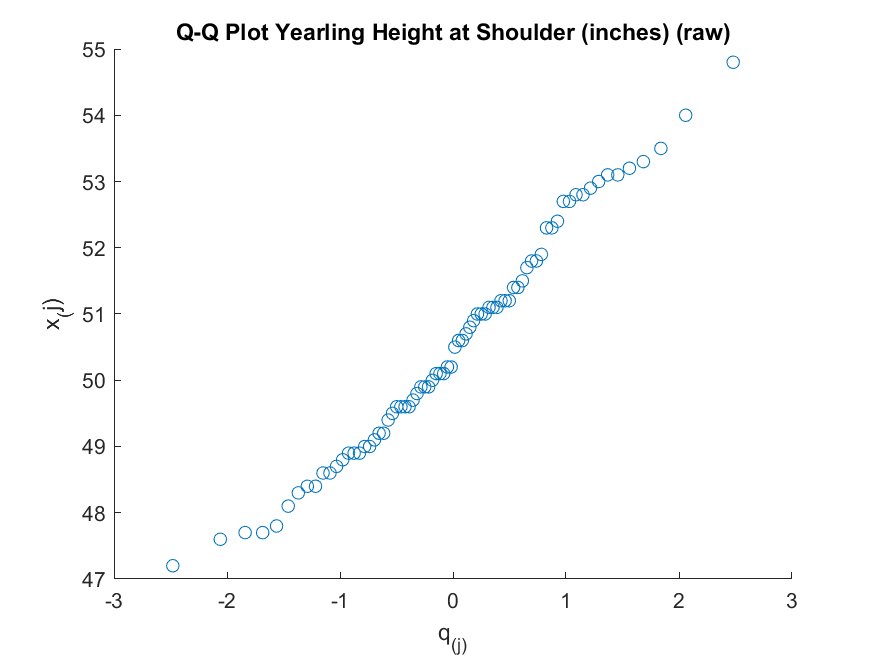
\includegraphics[scale=0.6]{./matlab/chapter-4/sol4.38.qq.1.png}
    \end{figure}
\end{center}

For ($x_{2}$), we're looking at the bull fat free body (pounds) for 76 valid observations. The simulated 0.01, 0.05, and 0.10 level critical correlation coefficient test values for a sample size of 76 are, 0.9772, 0.9839, and 0.9867, respectively. The Q-Q correlation coefficient using the raw data was 0.9631, so the data would not be considered normally distributed at the 0.05 and 0.10 levels.

The transformation suggested by Box-Cox power transformation was -2.1944, but I rounded that to -2.2, so $x_{2}^{\prime} = x_{2}^{-2.2}$.
The Q-Q correlation coefficient on the transformed data was 0.9937, which is larger than all three critical values, so the data is now considered normally distributed at all three levels.
Below are the results of the power transformation and the Q-Q plots of the raw and transformed data.
The original plot shows an outlier separated out. The Q-Q plot of the transformed data was able to make the data much more linear.

\begin{center}
    \begin{figure}[H]
        \centering
        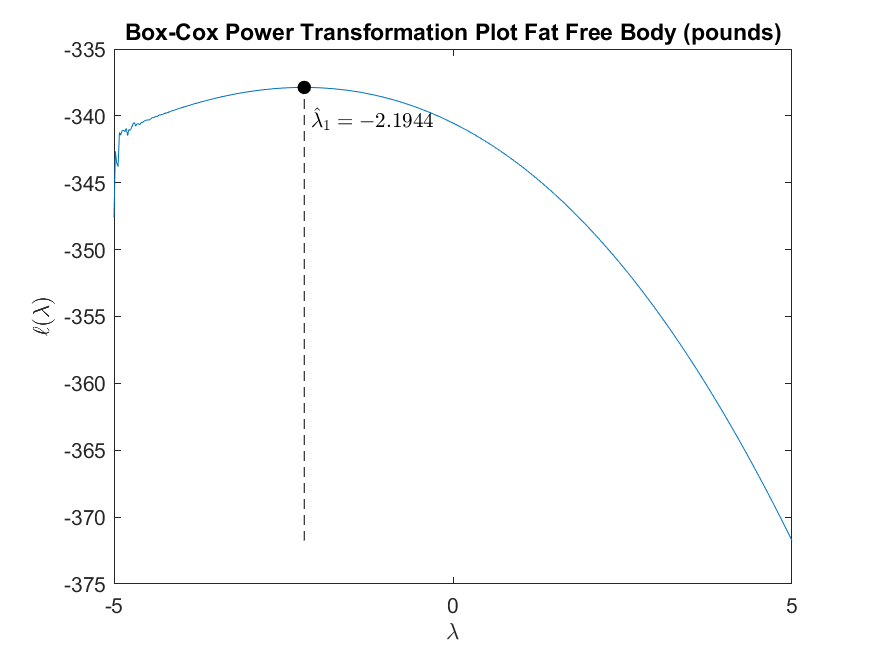
\includegraphics[scale=0.6]{./matlab/chapter-4/sol4.38.power.2.png}
    \end{figure}
\end{center}

\begin{center}
    \begin{figure}[H]
        \centering
        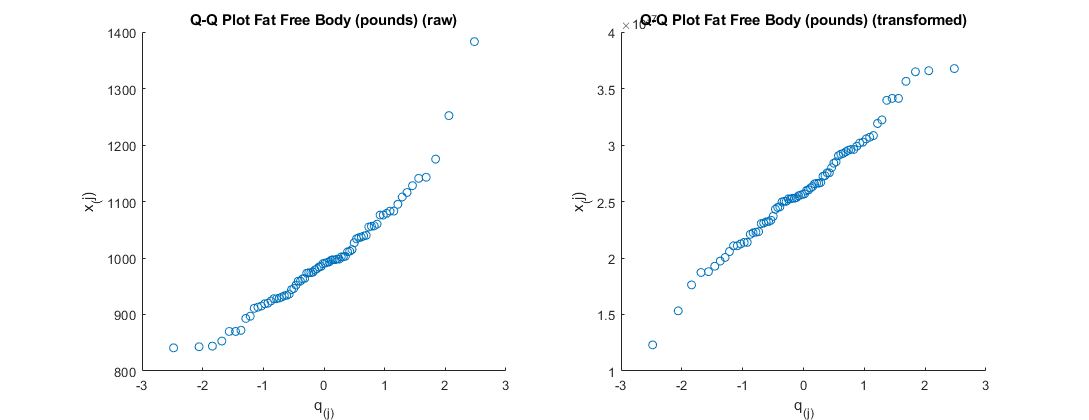
\includegraphics[scale=0.4]{./matlab/chapter-4/sol4.38.qq.2.png}
    \end{figure}
\end{center}

For ($x_{3}$), we're looking at the bull percent fat free body for 76 valid observations. The simulated 0.01, 0.05, and 0.10 level critical correlation coefficient test values for a sample size of 76 are, 0.9772, 0.9839, and 0.9867, respectively. The Q-Q correlation coefficient using the raw data was 0.9847, so the data would be considered normally distributed at the 0.01 and 0.05 levels, but not the 0.10 level.

The transformation suggested by Box-Cox power transformation was -3.477, but I rounded that to -3.5, so $x_{3}^{\prime} = x_{2}^{-3.5}$.
The Q-Q correlation coefficient on the transformed data was 0.9946, which is larger than all three critical values, so the data is now considered normally distributed at all three levels.
Below are the results of the power transformation and the Q-Q plots of the raw and transformed data.
The original plot shows a curvi-linear pattern, but the Q-Q plot of the transformed data was able to make the data much more linear.

\begin{center}
    \begin{figure}[H]
        \centering
        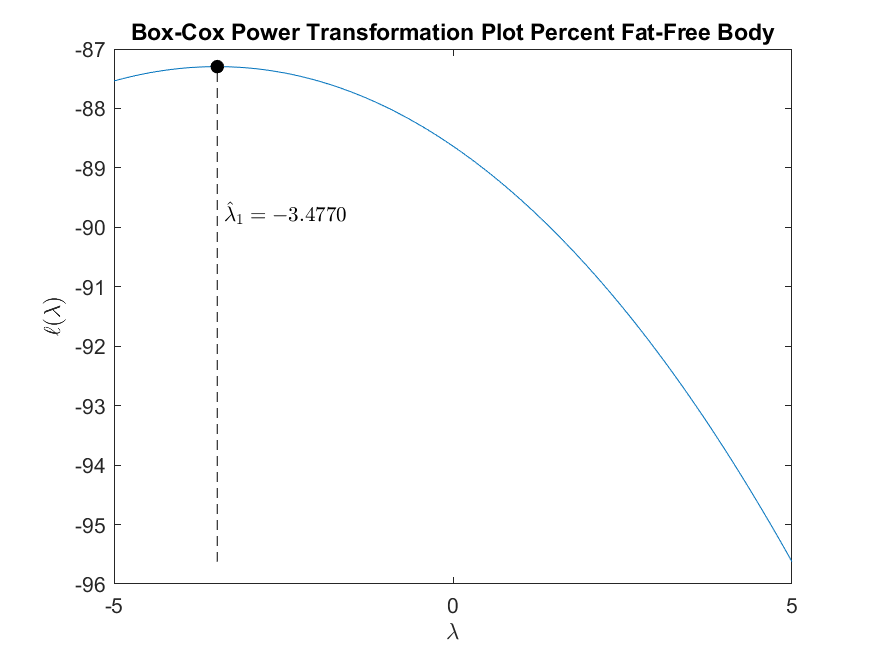
\includegraphics[scale=0.6]{./matlab/chapter-4/sol4.38.power.3.png}
    \end{figure}
\end{center}

\begin{center}
    \begin{figure}[H]
        \centering
        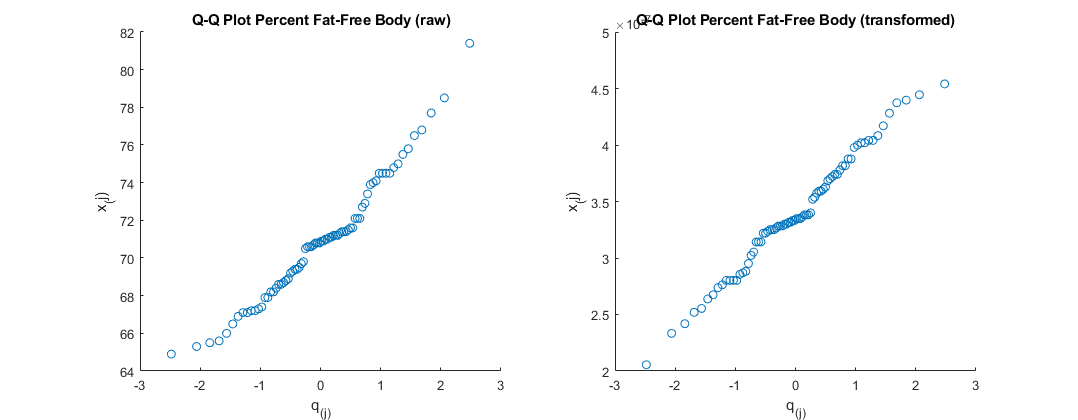
\includegraphics[scale=0.4]{./matlab/chapter-4/sol4.38.qq.3.png}
    \end{figure}
\end{center}

For ($x_{4}$), we're looking at the bull back fat (inches) for 76 valid observations. The simulated 0.01, 0.05, and 0.10 level critical correlation coefficient test values for a sample size of 76 are, 0.9772, 0.9839, and 0.9867, respectively. The Q-Q correlation coefficient using the raw data was 0.9376, less than any of the three critical values. Because of this the data would not be considered normally distributed at any of the three levels.

The transformation suggested by Box-Cox power transformation was -0.2906, but I rounded that to -0.3, so $x_{3}^{\prime} = x_{2}^{-0.3}$.
The Q-Q correlation coefficient on the transformed data was 0.96, which is an improvement, but not good enough to considered the data to be normally distributed.
Below are the results of the power transformation and the Q-Q plots of the raw and transformed data.
The data has lots of repeated values, so isn't exactly continuous. I don't think there'll be a common transformation to make this data normal. It might be better converted to a factor variable instead.

\begin{center}
    \begin{figure}[H]
        \centering
        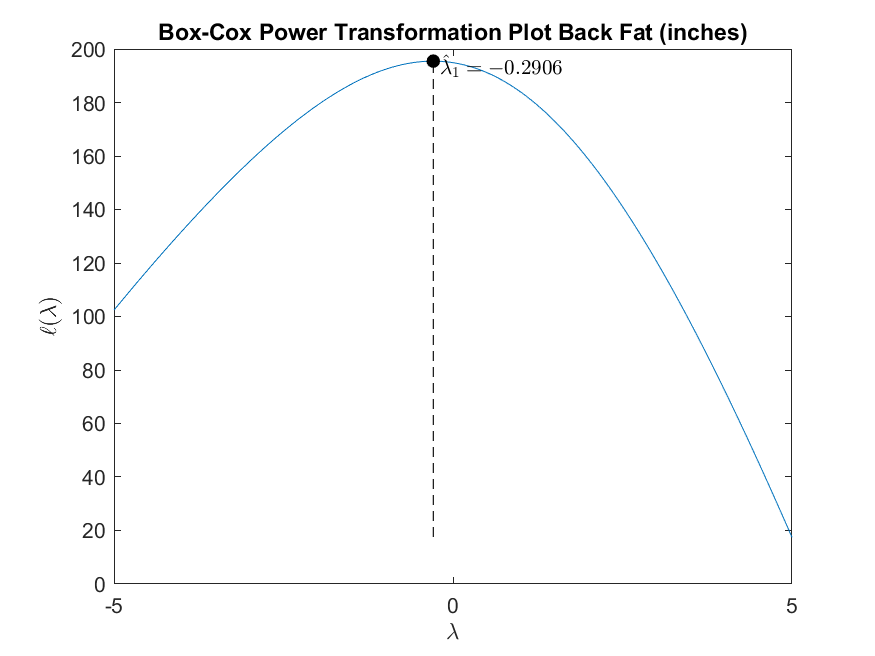
\includegraphics[scale=0.6]{./matlab/chapter-4/sol4.38.power.4.png}
    \end{figure}
\end{center}

\begin{center}
    \begin{figure}[H]
        \centering
        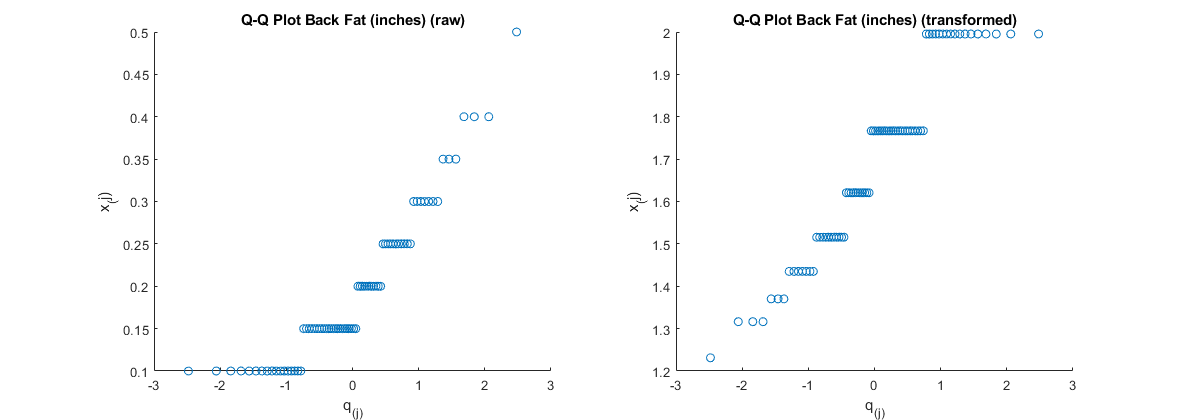
\includegraphics[scale=0.4]{./matlab/chapter-4/sol4.38.qq.4.png}
    \end{figure}
\end{center}

For ($x_{5}$), we're looking at the bull sale height at shoulder (inches) for 76 valid observations. The simulated 0.01, 0.05, and 0.10 level critical correlation coefficient test values for a sample size of 76 are, 0.9772, 0.9839, and 0.9867, respectively. The Q-Q correlation coefficient using the raw data is 0.9956, which is larger than all three of these values, so the data would be considered normally distributed at the 0.01, 0.05, and 0.10 levels.

We don't really need to transform the data, but just to see how much better it can get, the Box-Cox power transformation max was at 0.01, and rounded to 0, so $x_{5}^{\prime} = \ln\{x_{5}\}$. The Q-Q correlation coefficient on the transformed data was 0.9959, so we do get a slight improvement. Below is the Q-Q plot for the raw data, which looks really good.

\begin{center}
    \begin{figure}[H]
        \centering
        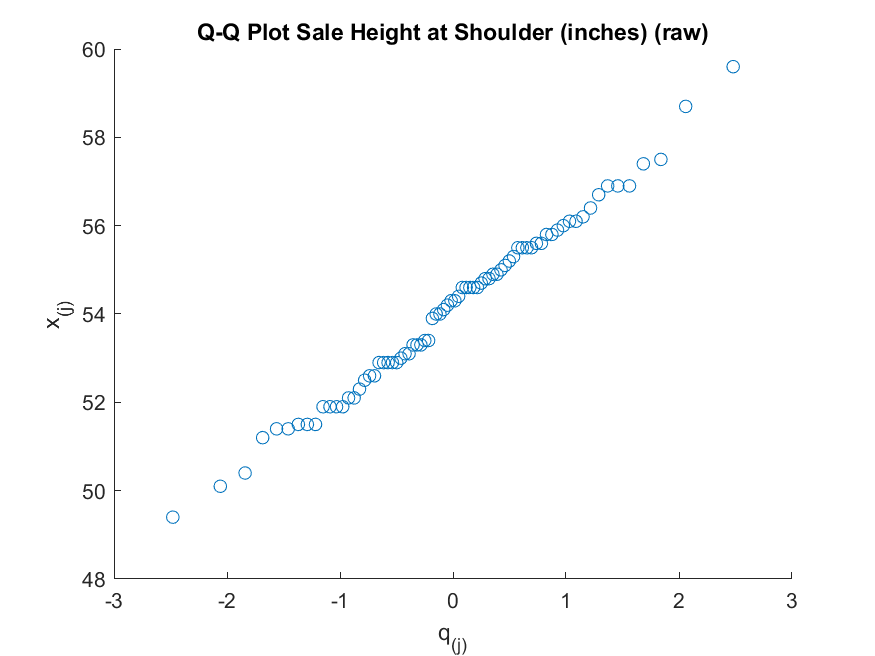
\includegraphics[scale=0.6]{./matlab/chapter-4/sol4.38.qq.5.png}
    \end{figure}
\end{center}

For ($x_{6}$), we're looking at the bull sale weight (pounds) for 76 valid observations. The simulated 0.01, 0.05, and 0.10 level critical correlation coefficient test values for a sample size of 76 are, 0.9772, 0.9839, and 0.9867, respectively. The Q-Q correlation coefficient using the raw data is 0.9956, which is larger than all three of these values, so the data would be considered normally distributed at the 0.01, 0.05, and 0.10 levels.

We don't really need to transform the data, but just to see how much better it can get, the Box-Cox power transformation max was at -0.6112, and rounded to -0.5, so $x_{6}^{\prime} = \frac{1}{\sqrt{x_{6}}}$. The Q-Q correlation coefficient on the transformed data was 0.9968, so we do get a slight improvement. Below is the Q-Q plot for the raw data, which looks really good.

\begin{center}
    \begin{figure}[H]
        \centering
        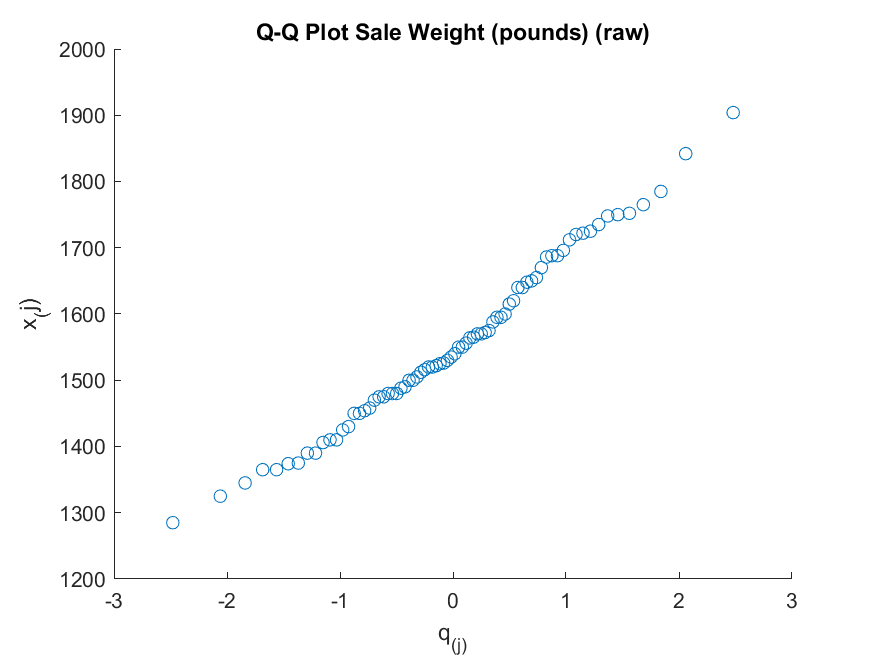
\includegraphics[scale=0.6]{./matlab/chapter-4/sol4.38.qq.6.png}
    \end{figure}
\end{center}

Computing the statistical distance based on our 6 covariates and creating a Chi-Squared plot (below). The raw data on the left shows two observations with statistical distances larger than most of the data. The transformed data on the right does show some improvement, but observation 15 has a larger statistical distance than the others (15.777). Without them the overall data would appear much more normal, but assuming it's not a measurement error, this observations will stay. Even with the outlier in the transformed data, it still looks fairly linear. I would think this data is multivariate normal.

\begin{center}
    \begin{figure}[H]
        \centering
        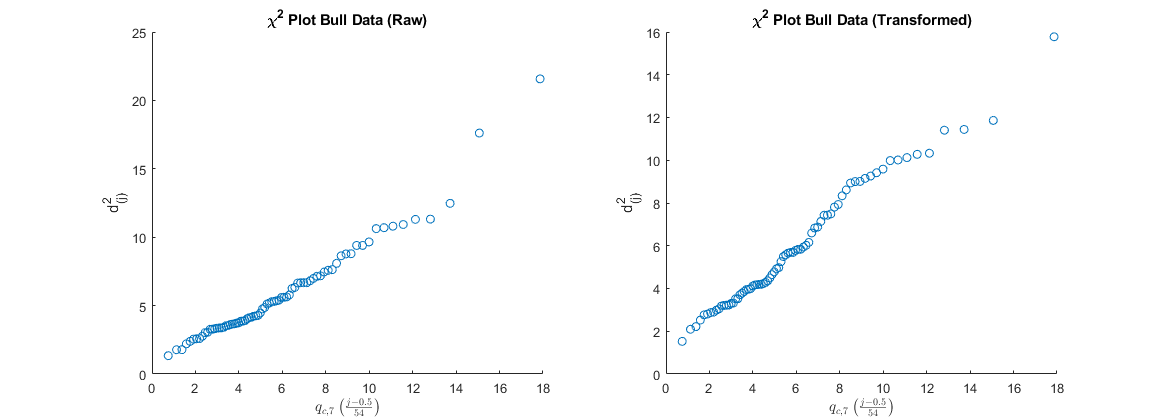
\includegraphics[scale=0.4]{./matlab/chapter-4/sol4.38.chi2.png}
    \end{figure}
\end{center}